\documentclass[20pt,margin=1in,innermargin=-4.5in,blockverticalspace=-0.25in]{tikzposter}
\geometry{paperwidth=42in,paperheight=30in}
\usepackage[utf8]{inputenc}
\usepackage{amsmath}
\usepackage{amsfonts}
\usepackage{amsthm}
\usepackage{amssymb}
\usepackage{mathrsfs}
\usepackage{graphicx}
\usepackage{adjustbox}
\usepackage{enumitem}
\usepackage[backend=biber,style=numeric]{biblatex}
\usepackage{emory-theme}

\usepackage{mwe} % for placeholder images

\addbibresource{refs.bib}

% set theme parameters
\tikzposterlatexaffectionproofoff
\usetheme{EmoryTheme}
\usecolorstyle{EmoryStyle}

\title{Preliminares Matemáticos}
\author{Pedro Villar}
\institute{Análisis Numérico - Primer Cuatrimestre 2024}	
\titlegraphic{\adjustbox{left=0.35\textwidth}{
\includegraphics[width=0.3\textwidth]{famaf-logo.jpg}}}

% begin document
\begin{document}
\maketitle
\centering
\begin{columns}
    \column{0.32}
    \block{Teorema del valor intermedio para funciones continuas}{
         Sea $f: [a,b] \to \mathbb{R}$ una función continua. Entonces, para todo $y$ entre $f(a)$ y $f(b)$, existe un $c$ en $[a,b]$ tal que $f(c) = y$.
         \begin{tikzfigure}[Teorema del valor intermedio.]
            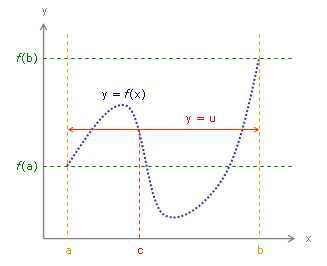
\includegraphics[width=0.6\linewidth]{valorme.png}
        \end{tikzfigure}
    }

    \block{Teorema del valor medio para funciones derivables}{
        Sea $f: [a,b] \to \mathbb{R}$ una función derivable. Entonces, existe un $c$ en $[a,b]$ tal que
        \begin{equation*}
            f'(c) = \frac{f(b) - f(a)}{b - a}.
        \end{equation*}
        \begin{tikzfigure}[Teorema del valor medio.]
            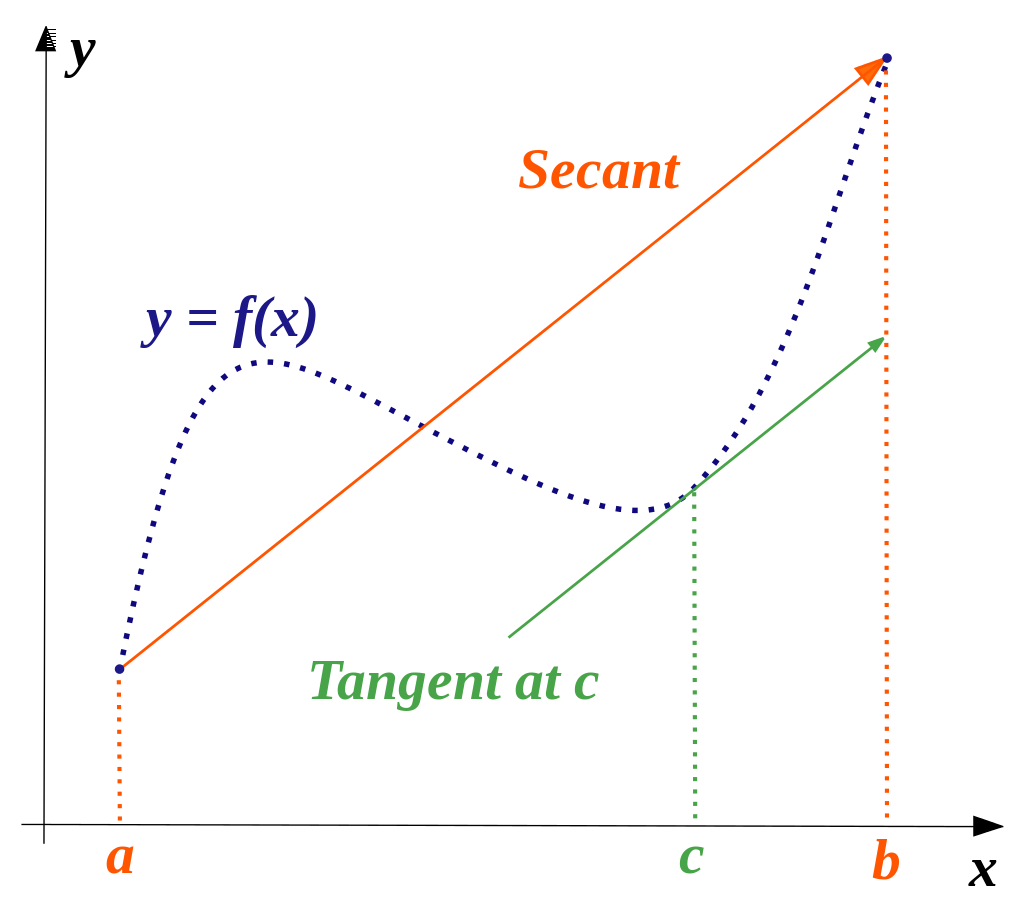
\includegraphics[width=0.6\linewidth]{valormedio.png}
        \end{tikzfigure}
    }

    \column{0.36}
    \block{Teorema de Taylor}{
        Si $f\in C^{(n)}[a,b]$ y existe $f^{n+1}(a,b)$ entonces para todo par $x,c \in [a,b]$ se tiene que 
        \begin{equation*}
            f(x) = \sum_{k=0}^{n} \frac{f^{(k)}(c)}{k!}(x-c)^k + E_n(x),
        \end{equation*}
        donde 
        \begin{equation*}
            E_n(x) = \frac{f^{(n+1)}(\xi)}{(n+1)!}(x-c)^{n+1}, \quad \xi \in (x,c).
        \end{equation*}
        \textbf{Observación:} tomando $y=c, (x-c)=h$ y por lo tanto $x = y+h$, entonces
        \begin{equation*}
            f(y+h) = f(y) + f'(y)h + \frac{f''(y)}{2}h^2 + \cdots + \frac{f^{(n)}(y)}{n!}h^n + E_n(h).
        \end{equation*}
        para algún $c \in (y,y+h)$.
    }

    \block{Teorema de Taylor del resto integral}{
        Si $f\in C^{(n+1)}[a,b]$ entonces para todo par $x,c \in [a,b]$ se tiene que 
        \begin{equation*}
            f(x) = \sum_{k=0}^{n} \frac{f^{(k)}(c)}{k!}(x-c)^k + R_n(x) 
        \end{equation*}
        donde 
        \begin{equation*}
            R_n(x) = \frac{1}{n!}\int_{c}^{x} f^{(n+1)}(t)(x-t)^ndt.
        \end{equation*}
    }

    \block{Sucesión convergente}{
        Una sucesión $\{x_n\}$ es convergente si existe un número $L$ tal que para todo $\varepsilon > 0$ existe un $N \in \mathbb{N}$ tal que si $n \ge N$ entonces $|x_n - L| < \varepsilon$.
    }

    \block{Convergencia lineal, superlineal y cuadrática}{
        Sea $\{x_n\}$ una sucesión convergente a $x_{ast}$.
        \begin{itemize}
            \item Se dice que la sucesión $\{x_n\}$ tiene tasa de convergencia (al menos) \textbf{lineal} si existe una constante $c$ tal que $0 < c < 1$ y un $N\in \mathbb{N}$ tal que
            \begin{equation*}
                |x_{n+1} - x_{\ast}|\leq c|x_n - x_{\ast}|, \quad \forall n \ge N.
            \end{equation*}
            \item Se dice que la tasa de convergencia es (al menos) \textbf{superlineal} si existe una sucesión $\{ \epsilon_n \}$ que converge a $0$ y un $N\in \mathbb{N}$ tal que
            \begin{equation*}
                |x_{n+1} - x_{\ast}| \leq \epsilon_n|x_n - x_{\ast}|, \quad \forall n \ge N.
            \end{equation*}
            \item Se dice que la tasa de convergencia es (al menos) \textbf{cuadrática} si existe una constante positiva $c$ y un $N\in \mathbb{N}$ tal que
            \begin{equation*}
                |x_{n+1} - x_{\ast}| \leq c|x_n - x_{\ast}|^2, \quad \forall n \ge N.
            \end{equation*}
        \end{itemize}
    }

    \column{0.32}
    \block{Notación $\mathcal{O}$ grande y $O$ chica}{
    Introducimos una notación para comparar sucesiones y funciones. Sean $\{ x_n \}$ y $\{ \alpha_n \}$ dos sucesiones. 
    \begin{itemize}
        \item Decimos que $$\{ x_n \}= \mathcal{O}(\alpha_n)$$ si existe una constante $C > 0$ y un $r \in \mathbb{N}$ tal que $$|x_n| \leq C|\alpha_n|, \quad \forall n \geq r.$$
        \item Decimos que $$\{ x_n \}= O(\alpha_n)$$ si existe una sucesión $\{ \varepsilon_n \}$ que converge a $0$, con $\varepsilon_n \ge 0$ y un $r \in \mathbb{N}$ tal que $|x_n| \leq \varepsilon_n|\alpha_n|, \quad \forall n \geq r.$
    \end{itemize}
    Esta notación también se puede extender a funciones. Se dice que
    \begin{equation*}
        f(x) = \mathcal{O}(g(x)) \quad \text{cuando} \quad x\to \infty
    \end{equation*}
    si existe una constante $C > 0$ y un $r \in \mathbb{R}$ tal que $|f(x)| \leq C|g(x)|, \quad \forall x \geq r$.
    Análogamente, se dice que
    \begin{equation*}
        f(x) = O(g(x)) \quad \text{cuando} \quad x\to \infty
    \end{equation*}
    si $\lim_{x\to \infty} \frac{f(x)}{g(x)} = 0$.
    }

    \block{Ejemplo de notación $O$ con sucesiones}{
        \begin{equation*}
            \frac{1}{n \cdot ln(n)} = O \left( \frac{1}{n} \right).
        \end{equation*} 
        Si
        \begin{equation*}
            \frac{1}{n \cdot ln(n)} \leq \varepsilon_n \left( \frac{1}{n} \right).
        \end{equation*}
        basta tomar $\varepsilon_n = \frac{1}{ln(n)}$.
    }

    \block{Ejemplo de notación $\mathcal{O}$ con funciones}{
        \begin{equation*}
            \sqrt{x^2 + 1} = \mathcal{O}(x) \quad \text{si} \quad x\to \infty.
        \end{equation*}
        pues
        \begin{equation*}
            \frac{\sqrt{x^2+1}}{x} = \sqrt{\frac{x^2+1}{x^2}} = \sqrt{1 + \frac{1}{x^2}} \leq C,
        \end{equation*}
        luego basta tomar $C=2$ y $r=1$.
    }
\end{columns}

%\begin{columns}
%    \column{0.5}
%    \block{Segunda Página}{
%        Contenido de la segunda página.
%    }
%
%    \column{0.5}
%    \block{Otro Bloque}{
%        Contenido de otro bloque en la segunda página.
%    }
%\end{columns}

\end{document}